\subsection{\acf*{WHOG}}
\label{sec:whitened_hog}

In 2012 Hariharan, Malik and Ramanan presented a technique \cite{Hariharan2012} to reduce the background clutter captured by \ac{HOG} called \acf{WHOG}. They proposed to apply a \ac{LDA} onto the \ac{HOG} features to increase their performance as similarity measures. The idea behind the approach is to gain similar effects as using a trained \ac{SVM} to remove background information by using a \ac{LDA} model, which requires a much lower train effort compared to a \ac{SVM}. As one can see, the fence in the \ac{HOG} representation in figure \ref{fig:whitened_hog:hog} partially hides the bicycle in the front. By training a \ac{SVM} the discriminative features of the bicycles can be weightened up as shown in figure \ref{fig:whitened_hog:svm}. As the usage of a \ac{SVM} is a rather time consuming task, the authors tried technologies used in earlier computer vision algorithms like the \ac{PCA} \cite{jolliffe2002principal} and \ac{LDA} as used in \cite{ahonen2006face}. The authors observed that a down projected feature space by a simple \ac{PCA} even decreases the performance in several PASCAL \cite{Pascal2007} classes compared to unmodified \ac{HOG} features. In general, a \ac{LDA} requires labeled information about the data which is going to be separated. This would make the approach very similar to a \ac{SVM} training and classification, including the required effort (notably training of a \ac{LDA} per image category). The authors were able to show that an one-time estimated background average $\mu_0$ and covariance matrix $\Sigma$ from unlabeled windows can be used for different categories. This fact is based on the assumption that the number of any one object is small compared to the total amount of windows and therefore a object independent $\mu_0$ can be estimated.

The authors also showed that their approach is also highly comparable to an ExemplarSVM classification, but with significantly faster train and run time. 

\begin{figure}
\begin{subfigure}[b]{0.4\textwidth}
\centering
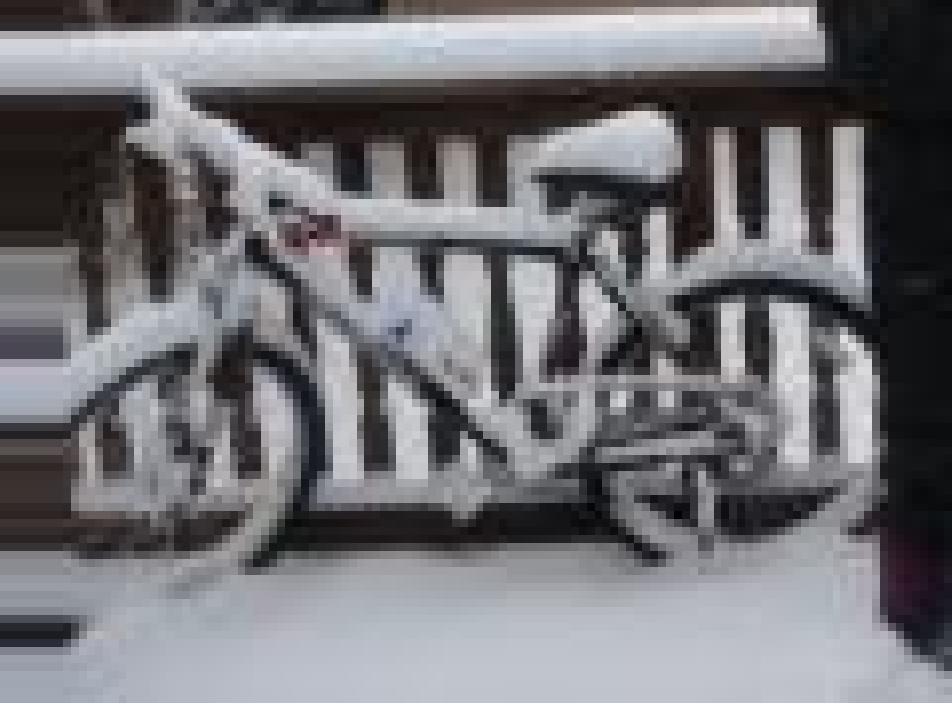
\includegraphics[width=\textwidth]{images/whitened_hog_image}
\caption[Image]{Image}
\label{fig:whitened_hog:image}
\end{subfigure}
%
\begin{subfigure}[b]{0.4\textwidth}
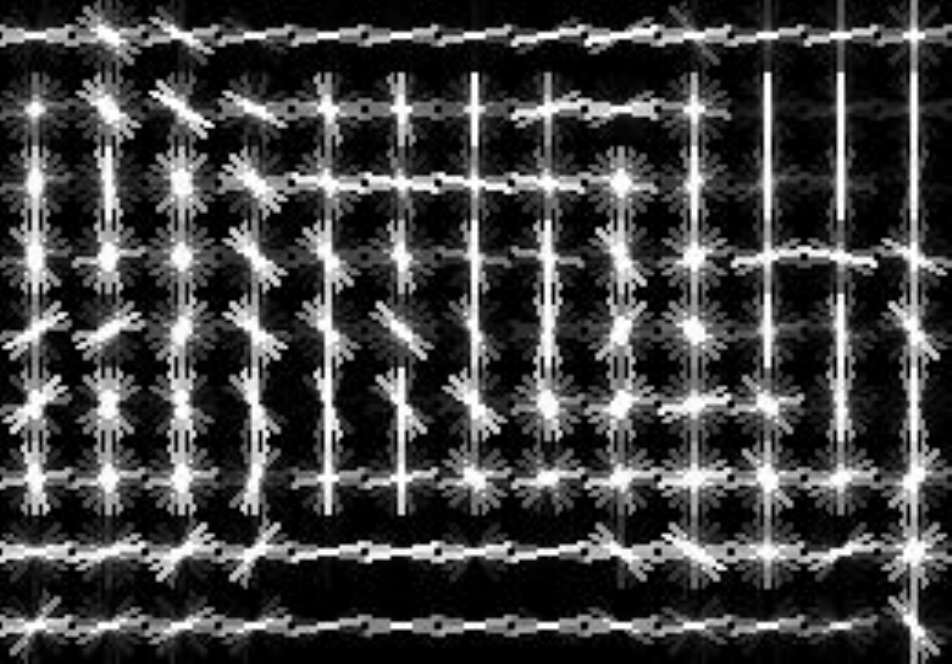
\includegraphics[width=\textwidth]{images/whitened_hog_hog}
\caption[HOG representation]{\acs{HOG} representation}
\label{fig:whitened_hog:hog}
\end{subfigure}

\begin{subfigure}[b]{0.3\textwidth}
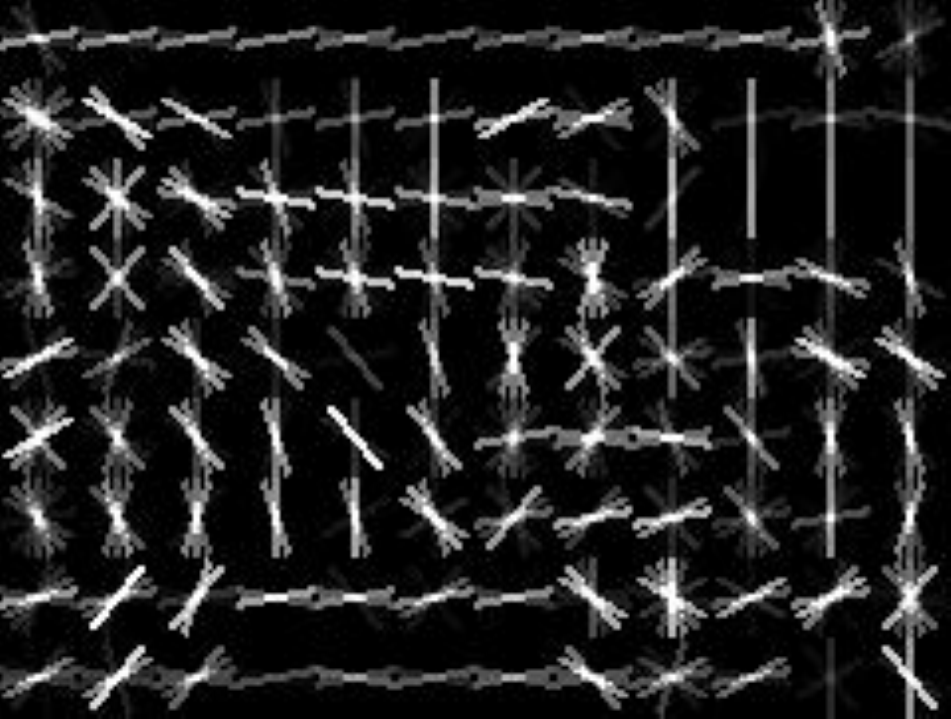
\includegraphics[width=\textwidth]{images/whitened_hog_svm}
\caption[SVM representation]{\acs{SVM} representation}
\label{fig:whitened_hog:svm}
\end{subfigure}
%
\begin{subfigure}[b]{0.3\textwidth}
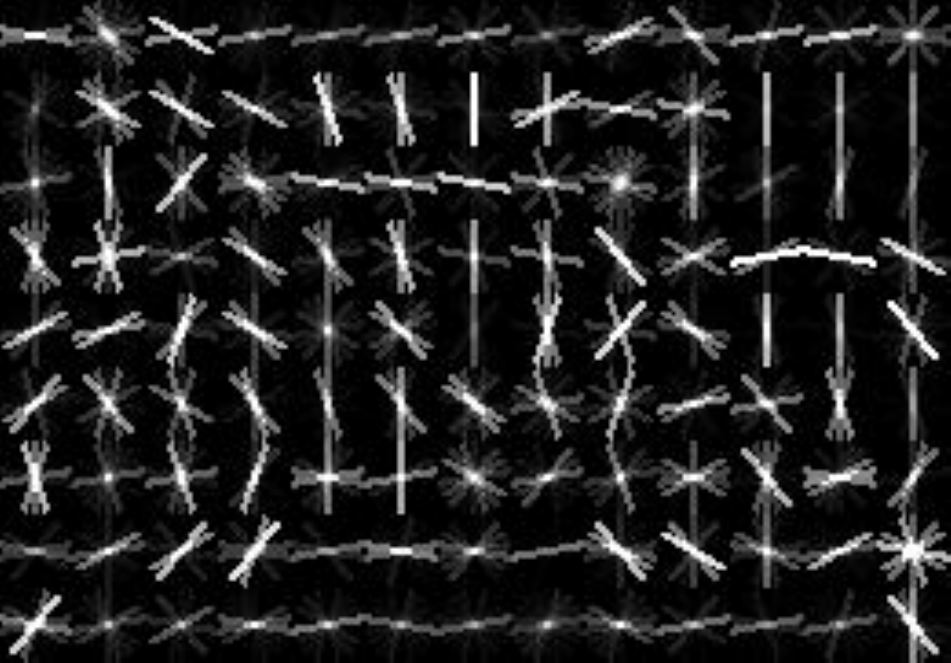
\includegraphics[width=\textwidth]{images/whitened_hog_lda}
\caption[LDA representation]{\acs{LDA} representation}
\label{fig:whitened_hog:lda}
\end{subfigure}
%
\begin{subfigure}[b]{0.3\textwidth}
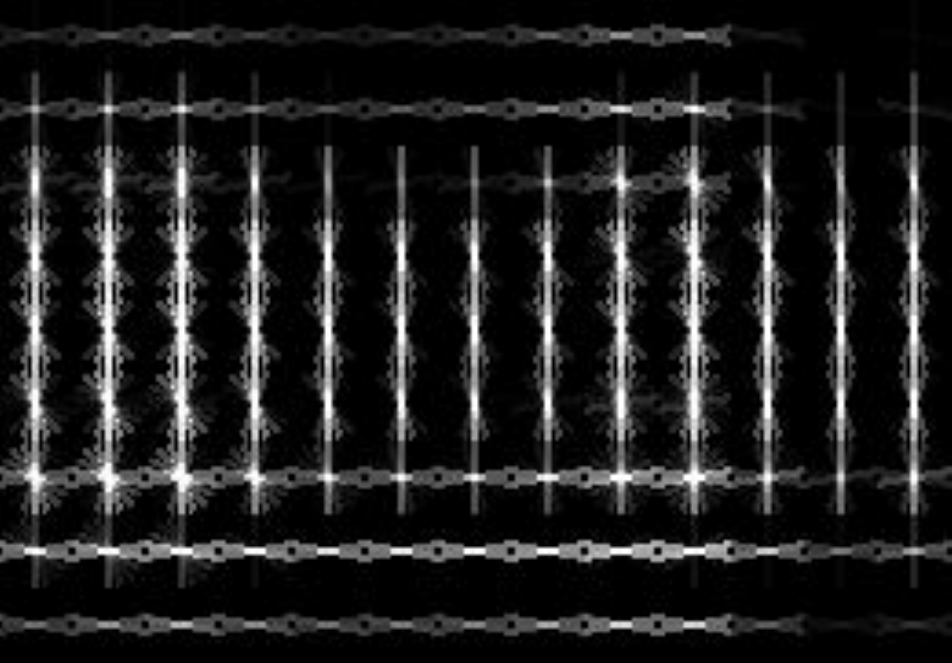
\includegraphics[width=\textwidth]{images/whitened_hog_pca}
\caption[PCA representation]{\acs{PCA} representation}
\label{fig:whitened_hog:pca}
\end{subfigure}
\caption{Bicycle in front of a fence, represented as \ac{HOG} features and weighted by different models.}
\label{fig:whitened_hog}
\end{figure}
